\documentclass[12pt,compress,aspectratio=169]{beamer}

\usetheme{metropolis}
\setbeamersize{text margin left=.5cm,text margin right=.5cm}

%\usepackage[utf8]{inputenc}
\usefonttheme{professionalfonts}
\usepackage{amsmath}
\usepackage{siunitx}
\usepackage{tikz}
\usepackage{mathpazo}
\usepackage{bm}
%\usepackage{hyperref}
\usepackage{mathtools}

\sisetup{
  detect-all,
  math-sf=\textsf,
  %number-math-rm=\textnormal,
  per-mode=symbol
}

\setsansfont{Roboto Light}
\setmonofont{Ubuntu Mono}
\setlength{\parskip}{0pt}
\setlength{\itemsep}{0pt}
\renewcommand{\baselinestretch}{1}


\title{Topic 1: Kinematics}
\subtitle{Advanced Placement Physics 1}
\author[TML]{Dr.\ Timothy Leung}
\institute{Olympiads School}
\date{\today}

\newcommand{\iii}{\ensuremath\hat{\bm{\imath}}}
\newcommand{\jjj}{\ensuremath\hat{\bm{\jmath}}}
\newcommand{\kkk}{\ensuremath\hat{\bm{k}}}
\newcommand{\pic}[2]{\includegraphics[width=#1\textwidth]{#2}}
\newcommand{\mb}[1]{\ensuremath\mathbf{#1}}
\newcommand{\eq}[2]{\vspace{#1}{\Large\begin{displaymath}#2\end{displaymath}}}
\newcommand{\magdir}[2]{#1\text{ [#2]}}

\begin{document}

\begin{frame}{}

  {\LARGE
    \begin{center}
      \textbf{WELCOME TO AP PHYSICS 1 \& 2}
    \end{center}
  }
\end{frame}



\begin{frame}{Pre-requisites}
  \begin{itemize}
  \item\textbf{Physics 11 and 12:} You will need to be comfortable with the
    topics covered in high-school level physics courses.
  \item\textbf{Vectors:} You need to be comfortable with vector operations,
    including addition and subtraction, multiplication/division by constants,
    as well as dot products and cross products.
  \end{itemize}
  If you already have a background in both differential and integral calculus,
  you may consider taking the AP Physics C exams instead.
\end{frame}



%\begin{frame}{AP Physics C Exams}
%  There are 2 AP Physics C exams, which are usually taken together on the same
%  day, in the first or second week of May of each year.
%  \begin{itemize}
%  \item Mechanics
%  \item Electricity and Magnetism
%  \end{itemize}
%  The Physics C exams are calculus based.
%\end{frame}



\begin{frame}{Classroom Rules}
  \begin{itemize}
  \item Treat each other with respect
  \item Raise your hands if you have a question. Don't wait too long
  \item E-mail me at \texttt{tleung@olympiadsmail.ca} for any questions related
    to physics and math and engineering
  \item Do \textbf{\emph{not}} try to find me on social media
  \end{itemize}
\end{frame}



\begin{frame}
  \titlepage
\end{frame}



\begin{frame}{Files for You to Download}
  \begin{itemize}
  \item\texttt{PhysAP1-courseOutline.pdf}--The course outline
%  \item\texttt{PhysAPC-equationSheet.pdf}--Equation sheet for your exams
  \item\texttt{PhysAP1-01-kinematics.pdf}--This set of slides
  %\item\texttt{PhysAP1-02-dynamics.pdf}--Slides for \emph{dynamics}, the next topic
  \item\texttt{PhysAP1-01-Homework.pdf}--Homework problems for kinematics
  %\item\texttt{PhysAP1-02-Homework.pdf}--Homework problems for dynamics
  \end{itemize}
%  
%  \vspace{.1in}Please download/print the PDF file for the class slides before
%  each class. There is no point copying notes that are already on the slides.
%  Instead, focus on things that aren't necessarily on the slides. If you wish
%  to print the slides, we recommend printing \emph{four} slides per page.
\end{frame}



%\begin{frame}{Vectors}
%  Please refer to the handout to make sure that you are familiar with basic
%  vector operations. We will be using a slightly more advanced notation method
%  for this course.
%\end{frame}



\section{Kinematics}

\begin{frame}{Kinematics}
  \textbf{Kinematics} is a discipline within mechanics concerning the
  mathematical description of the motion of bodies. It describes the
  relationships between 
  \begin{itemize}
  \item<alert@1> Position
  \item<alert@1> Displacement
  \item Distance 
  \item<alert@1> Velocity
  \item Speed
  \item<alert@1> Acceleration
  \end{itemize}
  Kinematics does not deal with the causes of motion. In the AP Physics 1 exam,
  kinematics account for approximately \SI{10}{\percent} to \SI{16}{\percent} of
  the marks.
\end{frame}



\begin{frame}{Position}
  \textbf{Position} ($\mb{x}$) describes the location of an object within a
  coordinate system. %The origin of the coordinate system is called the
  %``reference point''.
  The SI unit for position is \textbf{meter} (\si{\metre}).
  
  \eq{-.2in}{
    \mb{x}(t)=x(t)\iii + y(t)\jjj + z(t)\kkk
  }

  Vectors in 2D/3D Cartesian space are often expressed using the
  \textbf{IJK notation}
  \begin{itemize}
  \item $\iii$, $\jjj$ and $\kkk$ are \textbf{basis vectors} representing the
    directions of the $x$, $y$ and $z$ axes. Basis vectors are \textbf{unit
      vectors} (i.e.\ length 1)
  \item The IJK notation does not explicitly give the magnitude or the direction
    of the vector (needs to be calculated using the Pythagorean theorem)
  \end{itemize}
\end{frame}



\begin{frame}{Displacement}
  \textbf{Displacement} ($\Delta\mb{x}$) is the vector change in position from
  the initial position $\mb{x}_0$ within the same coordinate system. The unit
  for displacement is also meter.

  \eq{-.25in}{
      \Delta\mb{x}(t)=\mb{x}(t)-\mb{x}_0
      =(x-x_0)\iii + (y-y_0)\jjj + (z-z_0)\kkk
  }

  IJK notation makes vector addition and subtraction less prone to errors
 % \item Since the reference point $\mb{x}_{\text{ref}}=\mb{0}$, the position
 %   vector $\mb{x}$ is also its displacement from the reference point
%  \end{itemize}
\end{frame}



\begin{frame}{Distance}
  \textbf{Distance} $s$ is a quantity that is \emph{related} to displacement.
  It is:
  \begin{columns}
    \column{.7\textwidth}
    \begin{itemize}
    \item The length of the path taken by an object when it from $\mb{x}_0$ to
      $\mb{x}$
    \item A scalar quantity
    \item Always positive, i.e.\ $s\geq 0$
    \item Although the magnitude of the displacement vector is also a scalar,
      it is not necessarily the same as distance
    \item $s\geq |\Delta\mb{x}|$
    \end{itemize}
    
    \column{.3\textwidth}
    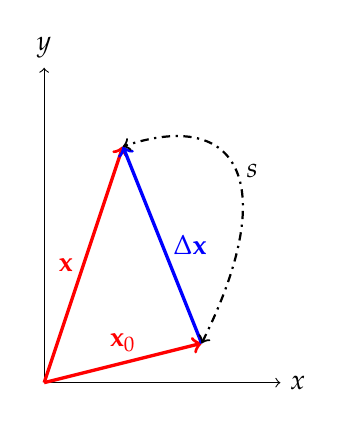
\begin{tikzpicture}[scale=.5]
      \draw[->](0,0)--(6,0) node[pos=1,right]{$x$};
      \draw[->](0,0)--(0,8) node[pos=1,above]{$y$};
      \draw[->,red,very thick] (0,0)--(4,1) node[midway,above]{$\mb{x}_0$};
      \draw[->,red,very thick] (0,0)--(2,6) node[midway,left]{$\mb{x}$};
      \draw[->,blue,very thick](4,1)--(2,6) node[midway,right]{$\Delta\mb{x}$};
      \draw[thick,dash dot,<->] (4,1)..controls (6,5) and (5,7)..(2,6)
      node[midway,right]{$s$};
    \end{tikzpicture}
  \end{columns}
  \vspace{.15in}Pay close attention to the difference between distance and displacement.
\end{frame}




%
%
%
%\begin{frame}{Integrating Velocity to Get Position/Displacement}
%  Conversely, if $\mb{v}(t)$ is the time rate of change of position
%  $\mb{x}(t)$, then $\mb{x}$ is the time integral of $\mb{v}$:
%  
%  \eq{-.2in}{
%    \mb{x}(t)=\int\mb{v}(t)dt + \mb{x}_0
%  }
%  
%  The constant of integration $\mb{x}_0$ is the \emph{initial position} at
%  $t=0$. We can integrate each component to get $\mb{x}$:
%
% \eq{-.2in}{ \mb{x}(t)= \left(
%    \int v_x\bm{\hat{\imath}} +
%    \int v_y\bm{\hat{\jmath}} +
%    \int v_z\bm{\hat{k}}
%    \right) dt + \mb{x}_0
%  }
%\end{frame}



\begin{frame}{Average Velocity}
  \textbf{Average velocity} $\overline{\mb{v}}$ of an object is its
  displacement $\Delta\mb{x}$ over a \emph{finite} time interval $\Delta t$.
  The unit for velocity is \textbf{meters per second} (\si{\metre\per\second}):

  \eq{-.2in}{
    \boxed{
      \overline{\mb{v}}= \frac{\Delta\mb{x}}{\Delta t}
    }
  }
  
  Since the $\iii$, $\jjj$ and $\kkk$ directions ($x$, $y$, $z$ axes) are
  \emph{linearly independent}\footnote{mathematical way of saying that what happens in
  one axis does not affect another}, each component of average velocity can be
  calculated by separating each direction:

  \eq{-.2in}{
    \boxed{
      \overline{\mb{v}}=
      \frac{\Delta x}{\Delta t}\iii + \frac{\Delta y}{\Delta t}\jjj +
      \frac{\Delta z}{\Delta t}\kkk
    }
  }

  (Note: A bar is drawn over the symbol if it is averaged over time.)
  \vspace{.15in}
\end{frame}



\begin{frame}{Instantaneous Velocity}
  If displacement $d\mb{x}$ is calculated a very small\footnote{In
    calculus, a very small change is called \emph{infinitesimally small}} time
  interval $dt$, then velocity is called the \textbf{instantaneous velocity}:
  
  \eq{-.2in}{
	\overline{\mb{v}}= \frac{\Delta\mb{x}}{\Delta t}\quad\rightarrow\quad
	\boxed{\mb{v}= \frac{d\mb{x}}{dt}}
  }
  
  The instantaneous velocity is the slope of the tangent on the position-time graph.
\end{frame}



\begin{frame}{Instantaneous \& Average Speed}
  \textbf{Average speed} is similar to average velocity: it is the distance $s$
  traveled over a finite time interval $\Delta t$. Since distance is always
  positive, so too is the average speed
 
  \eq{-.2in}{
    \boxed{\overline{v}=\frac{s}{\Delta t}}
  }

  Likewise, when the time interval is made infinitesimally small, then the speed is
  called the \textbf{instantaneous speed} $v$. Instantaneous speed $v$ is the
  magnitude of the instantaneous velocity vector.
\end{frame}



%\begin{frame}{Path}
%  Sometimes instead of explicitly describing the position $x=x(t)$ and $y=y(t)$,
%  the path of an object can be given in terms of $x$ coordinate $y=y(x)$, while
%  giving the $x$ (or $y$) coordinate as a function of time.
%  \begin{itemize}
%  \item In this case, substitute the expression for $x(t)$ into $y=y(x)$ to
%    get an expression of $y=y(t)$
%  \item Take derivative using chain rule to get $v_y=v_y(t)$
%  \end{itemize}
%\end{frame}


\begin{frame}{Instantaneous \& Average Acceleration}
  In the same way that velocity describes how quickly position changes with time, 
  \textbf{average acceleration} $\overline{\mb{a}}$ is the change in velocity
  $\Delta\mb{v}$ over a finite time interval $\Delta t$. The unit for
  acceleration is \textbf{meters per second squared}
  (\si{\metre\per\second\squared}).

  \eq{-.1in}{
    \boxed{
      \overline{\mb{a}} = \frac{\Delta\mb{v}}{\Delta t}
      =\frac{\mb{v}(t)-\mb{v}(t_0)}{t-t_0}
    }
  }
  
  Making the time interval $\Delta t=t-t_0$ infinitesimally small gives the
  \textbf{instantaneous acceleration} $\mb{a}(t)$.
\end{frame}



%\begin{frame}{Special Notation}{When Differentiating With Time}
%  Physicists and engineers often use a special notation when the derivative is
%  taken with respect to \emph{time}, by writing a dot above the variable:
%  \begin{itemize}
%  \item Velocity:
%
%    \eq{-.25in}{
%      \mb{v}(t)= \dot{\mb{x}}
%    }
%  \item Acceleration:
%
%    \eq{-.25in}{
%      \mb{a}(t)= \dot{\mb{v}}=\ddot{\mb{x}}
%    }
%  \end{itemize}
%  We will use this notation whenever it is convenient
%\end{frame}
%
%
%
%\begin{frame}{Integrating Acceleration to Get Velocity}
%  Velocity $\mb{v}(t)$ is the time integral of acceleration $\mb{a}(t)$:
%    
%  \eq{-.2in}{
%    \mb{v}(t)=\int\mb{a}(t)dt+\mb{v}_0
%  }
%
%  Again, we can integrate each component of the vector independently:
%
%  \eq{-.2in}{
%    \mb{v}(t)=
%    \left(\int a_x\bm{\hat{\imath}} +
%    \int a_y\bm{\hat{\jmath}} +
%    \int a_z\bm{\hat{k}}\right) dt +\mb{v}_0
%  }
%\end{frame}



\begin{frame}{If You Are Curious (Not Part of AP Physics)}
  For the curious minds, the time rate of change of acceleration is called
  \textbf{jerk}, with a unit of \si{\metre\per\second^3}:

  \eq{-.25in}{
    \overline{\mb{j}}= \frac{\Delta\mb{a}}{\Delta t}
  }

  The time rate of change in jerk is called \textbf{jounce} or \textbf{snap},
  with a unit of \si{\metre\per\second^4}:
  
  \eq{-.1in}{
    \overline{\mb{s}}=\frac{\Delta\mb{j}}{\Delta t}
  }
  
  The next motion quantities are are called \textbf{crackle} and \textbf{pop},
  but these quantities are almost never used.\vspace{.3in}
\end{frame}



\begin{frame}{Acceleration as Functions of Velocity and Position}
  Sometimes, acceleration are expressed as a function of velocity or position
  rather than of time, depending on the forces acting on them. For example:
  \begin{itemize}
  \item Gravitational or electrostatic forces: $a(x)=Ax^{-2}$
  \item Spring force: $\displaystyle a(x)=-Bx$
  \item Damping force (e.g.\ shock absorbers): $a(v)=Cv$
  \item Aerodynamic drag: $a(v)=Dv^2$
  \end{itemize}
  In these cases, solving for the motion quantities $x(t)$, $v(t)$ and $a(t)$
  may require calculus, numerical integration methods, or the conservation of
  energy.
\end{frame}



\section{Kinematic Equations}

\begin{frame}{Kinematic Equations}
  Without calculus, kinematic problems in AP Physics 1 only deal with
  \underline{constant acceleration}.
  %Non-constant acceleration problems are studied in depth in Physics C.
  The 1D kinematic equations that will be used in Physics 1 are:
  \begin{columns}
    \column{.45\textwidth}

    \vspace{-.3in}{\Large
      \begin{align*}
        x &= x_0+ v_0t + \frac12at^2\\
        v &= v_0+at\\
        v^2 &= v_0^2+ 2a(x-x_0)
      \end{align*}
    }
    
    \column{.55\textwidth}
    \begin{itemize}
    \item Initial position: $x_0$
    \item Position at time $t$: $x$
    \item Initial velocity: $v_0$
    \item Velocity at time $t$: $v$
    \item Acceleration (constant): $a$
    \end{itemize}
  \end{columns}
  These equations are sometimes called the ``Big-five'' or ``Big-four''
  in Grade 11/12 Physics. In AP, you are given only 3 equations in your
  equation sheet.
\end{frame}


%\begin{frame}{Non-Constant Acceleration}
%  What happens when acceleration is not constant? Our options are:
%  \begin{itemize}
%  \item Give up (bad idea!)
%  \item Use calculus
%  \item Use a numerical iterative method
%  \item<alert@1>Use conservation of energy
%  \end{itemize}
%\end{frame}

\section{Motion Graphs}

\begin{frame}{Motion Graphs}
  You should already be familiar with the \emph{basic} 1D motion graphs.
  These are still used in AP Physics.
  \begin{itemize}
  \item Position vs.\ time ($x$-$t$) graph
  \item Velocity vs.\ time ($v$-$t$) graph
  \item Acceleration vs.\ time ($a$-$t$) graph
  \end{itemize}
  %Note that these graphs are only valid for 1D motion. Think of them as
  They are the graphical representation of the kinematic equations from the
  previous slide.
  %Depending on the situation, it may be more useful to plot motion
  %using other quantities as well.
\end{frame}



\begin{frame}{Uniform Motion}
  An object moves with constant velocity
  (neither magnitude nor direction changes) and therefore no acceleration.
  \begin{center}
    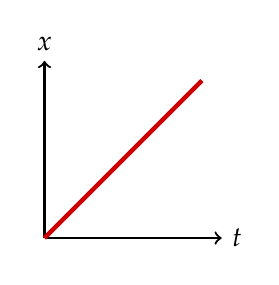
\begin{tikzpicture}[scale=.5]
      \draw[->,thick] (0,0)--(4.5,0) node[pos=1,right]{$t$};
      \draw[->,thick] (0,0)--(0,4.5) node[pos=1,above]{$x$};
      \draw[red!80!black,ultra thick](0,0)--(4,4);
    \end{tikzpicture}
    \hspace{.15in}
    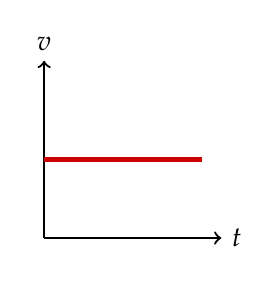
\begin{tikzpicture}[scale=.5]
      \draw[->,thick] (0,0)--(4.5,0) node[pos=1,right]{$t$};
      \draw[->,thick] (0,0)--(0,4.5) node[pos=1,above]{$v$};
      \draw[red!80!black,ultra thick](0,2)--(4,2);
    \end{tikzpicture}
    \hspace{.15in}
    \begin{tikzpicture}[scale=.5]
      \draw[->,thick] (0,0)--(4.5,0) node[pos=1,right]{$t$};
      \draw[->,thick] (0,0)--(0,4.5) node[pos=1,above]{$a$};
      \draw[red!80!black,ultra thick](0,0)--(4,0);
    \end{tikzpicture}
  \end{center}
  \begin{itemize}
  \item Constant velocity has a straight line in the $x$-$t$ graph
  \item The slope of the $x$-$t$ graph is the velocity $v$, which is constant
  \item The slope of the $v$-$t$ graph is the acceleration $a$, which is zero by
    definition
  \end{itemize}
\end{frame}



\begin{frame}{Uniform Acceleration}
  An object moves with a constant non-zero acceleration:
  \begin{center}
    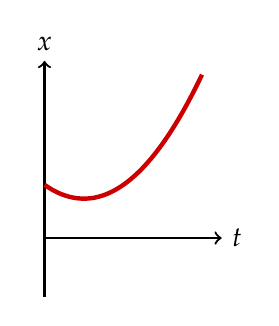
\begin{tikzpicture}[scale=.5]
      \draw[->,thick] (0,0)--(4.5,0) node[pos=1,right]{$t$};
      \draw[->,thick] (0,-1.5)--(0,4.5) node[pos=1,above]{$x$};
      \draw[smooth,samples=20,domain=0:4,red!80!black,ultra thick]
      plot({\x},{0.35*(\x-1)*(\x-1)+1});
    \end{tikzpicture}
    \hspace{.15in}
    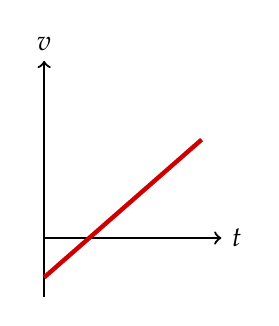
\begin{tikzpicture}[scale=.5]
      \draw[->,thick] (0,0)--(4.5,0) node[pos=1,right]{$t$};
      \draw[->,thick] (0,-1.5)--(0,4.5) node[pos=1,above]{$v$};
      \draw[red!80!black,ultra thick](0,-1)--(4,2.5);
    \end{tikzpicture}
    \hspace{.15in}
    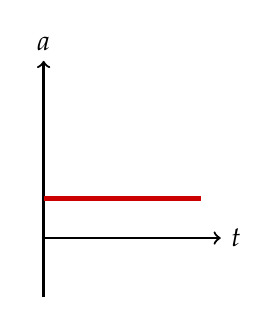
\begin{tikzpicture}[scale=.5]
      \draw[->,thick] (0,0)--(4.5,0) node[pos=1,right]{$t$};
      \draw[->,thick] (0,-1.5)--(0,4.5) node[pos=1,above]{$a$};
      \draw[red!80!black,ultra thick](0,1)--(4,1);
    \end{tikzpicture}
  \end{center}
  \begin{itemize}
  \item The $x$-$t$ graph is part of a \emph{parabola}
    \begin{itemize}
    \item If the parabola is \emph{convex} (opens up), acceleration is ($+$)
    \item If the parabola is \emph{concave} (opens down), acceleration is ($-$)
    \end{itemize}
  \item The $v$-$t$ graph is a straight line; its slope (a constant) is the
    acceleration
  \item The $a$-$t$ graph is a horizontal straight line
  \end{itemize}
\end{frame}



\begin{frame}{Simple Harmonic Motion}
  For \textbf{harmonic motions} (vibrations, oscillations), $x$, $v$ and $a$
  are all non-constant, and they all change with time as sinusoidal functions.
  %Although we cannot use the kinematic equations here, we will be studying
  %this motion in the course.
  \begin{center}
    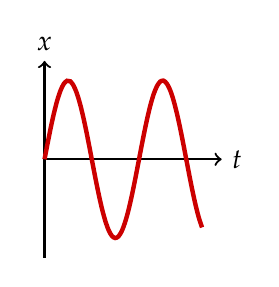
\begin{tikzpicture}[scale=.5]
      \draw[->,thick] (0,0)--(4.5,0) node[pos=1,right]{$t$};
      \draw[->,thick] (0,-2.5)--(0,2.5) node[pos=1,above]{$x$};
      \draw[smooth,samples=50,domain=0:4,red!80!black,ultra thick]
      plot({\x},{2*sin(150*\x)});
    \end{tikzpicture}
    \hspace{.15in}
    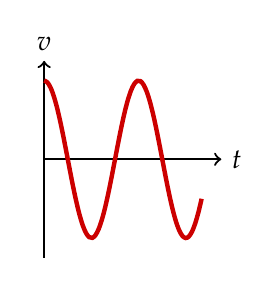
\begin{tikzpicture}[scale=.5]
      \draw[->,thick] (0,0)--(4.5,0) node[pos=1,right]{$t$};
      \draw[->,thick] (0,-2.5)--(0,2.5) node[pos=1,above]{$v$};
      \draw[smooth,samples=50,domain=0:4,red!80!black,ultra thick]
      plot({\x},{2*cos(150*\x)});
    \end{tikzpicture}
    \hspace{.15in}
    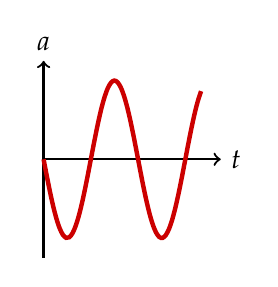
\begin{tikzpicture}[scale=.5]
      \draw[->,thick] (0,0)--(4.5,0) node[pos=1,right]{$t$};
      \draw[->,thick] (0,-2.5)--(0,2.5) node[pos=1,above]{$a$};
      \draw[smooth,samples=50,domain=0:4,red!80!black,ultra thick]
      plot({\x},{-2*sin(150*\x)});
    \end{tikzpicture}
  \end{center}
  \textbf{Bottom line}: regardless of the type motion,
  \begin{itemize}
  \item The $v$-$t$ graph is the slope of the $x$-$t$ graph
  \item The $a$-$t$ graph is the slope of the $v$-$t$ graph
  \end{itemize}
\end{frame}



\begin{frame}{Area Under Motion Graphs}
  \begin{columns}
    \column{.25\textwidth}
    \begin{center}
      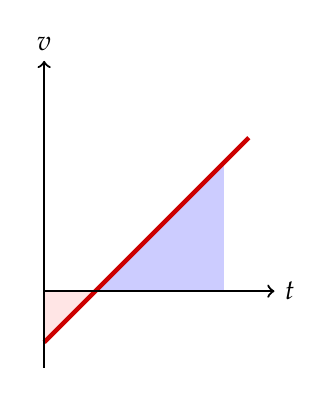
\begin{tikzpicture}[scale=.65]
        \draw[pink!40,fill=pink!40](0,0)--(0,-1)--(1,0)--cycle;
        \draw[blue!20,fill=blue!20](1,0)--(3.5,0)--(3.5,2.5)--cycle;
        \draw[red!80!black,ultra thick](0,-1)--(4,3);
        \draw[->,thick] (0,0)--(4.5,0) node[pos=1,right]{$t$};
        \draw[->,thick] (0,-1.5)--(0,4.5) node[pos=1,above]{$v$};
      \end{tikzpicture}
    \end{center}
    
    \column{.75\textwidth}
    The area under the $v$-$t$ graph is the displacement $\Delta x$:
    \begin{itemize}
    \item Area \textcolor{blue!20}{\emph{above}} the time axis: $+$
      displacement
    \item Area \textcolor{red!40}{\emph{below}} the time axis: $-$ displacement
    \end{itemize}
    \vspace{.1in}The area under the $a$-$t$ graph is the change in velocity
    $\Delta v$:
    \begin{itemize}
    \item Area \emph{above} the time axis: $+$ change in velocity
    \item Area \emph{below} the time axis: $-$ change in velocity
    \end{itemize}

    \vspace{.1in}The area under the $x$-$t$ graph has no physical meaning.
  \end{columns}
\end{frame}



\begin{frame}{Velocity Squared vs.\ Displacement}
  If velocity information is given as a function of position\footnote{Depends
    on experimental set up} then a motion graph can be plotted using this
  kinematic equation:

  \eq{-.2in}{
    \underbracket{v^2}_y=\underbracket{v_0^2}_b+\underbracket{2a}_m
    \underbracket{(x-x_0)}_x
  }

  by plotting $v^2$ on the $y$-axis and displacement $\Delta x=x-x_0$ on the
  $x$-axis. The slope of the graph is $m=2a$. The square of the initial
  velocity ($v_0^2$) is the $y$-intercept.
\end{frame}



\begin{frame}{Graphing ``Linear'' Functions}
  This concept extends to graphing other physical quantities not relating to
  motion:
  \begin{itemize}
  \item To find the index of refraction of a material using Snell's law, plot
    $\sin\theta_i$ vs.\ $\sin\theta_2$ (rather than $\theta_1$ vs.\ $\theta_2$).
    The slope is the index $n$:

    \eq{-.25in}{
      \underbracket{\sin\theta_1}_y=\underbracket{n}_m
      \underbracket{\sin\theta_2}_x
    }
  \item To relate the period of oscillation of a simple pendulum to the length
    of the pendulum, plot $T$ vs.\ $\sqrt{L}$:

    \eq{-.2in}{
      \underbracket{T}_y=\underbracket{\frac{2\pi}{\sqrt{g}}}_m
      \underbracket{\sqrt{L}}_x
    }
  \end{itemize}
\end{frame}

\section{Projectile Motion}

\begin{frame}{Projectile Motion}
  A \textbf{projectile} is an object that is launched with an initial velocity
  of $\mb{v}_0$ along a parabolic trajectory and accelerates only due to
  gravity.
  \begin{center}
    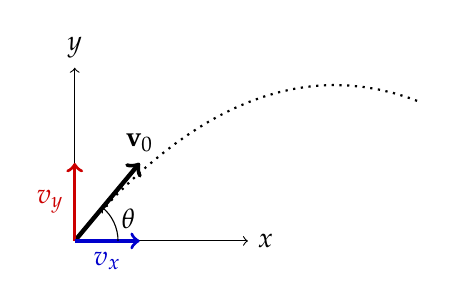
\begin{tikzpicture}[scale=1.1]
      \draw[->](0,0)--(2,0) node[pos=1,right]{$x$};
      \draw[->](0,0)--(0,2) node[pos=1,above]{$y$};
      \draw[dotted,domain=0:4,thick] plot (\x, {1.2*\x-.2*\x*\x});
      \draw[ultra thick,->](0,0)--(.75,.9)node[pos=1,above]{$\mb{v}_0$};
      \draw[very thick,red!80!black,->]
      (0,0)--(0,.9)node[midway,left]{$v_y$};
      \draw[very thick,blue!80!black,->]
      (0,0)--(.75,0)node[midway,below]{$v_x$};
      \draw[->](.5,0)arc(0:52:.5) node[pos=.6,right]{$\theta$};
    \end{tikzpicture}
  \end{center}
  \begin{itemize}
  \item $x$-axis: \emph{horizontal}, pointing \emph{forward}
  \item $y$-axis: \emph{vertical}, pointing \emph{up}
  \item Angle $\theta$ measured \emph{above} the horizontal
  \item The origin is usually where the projectile is launched
  %\item Consistent with the right-handed Cartesian coordinate system
  \end{itemize}
\end{frame}



\begin{frame}{Horizontal Direction}
  The initial velocity $\mb{v}_0$ can be decomposed into its $x$ and $y$
  components using the launch angle $\theta$:

  \eq{-.2in}{
    \mb{v}_0=v_x\iii + v_y\jjj =
    \left[v_0\cos\theta\right]\iii + \left[v_0\sin\theta\right]\jjj
  }

  There is no horizontal acceleration (i.e.\ $a_x=\num{0}$), therefore $v_x$ is
  constant. The kinematic equations reduce to a single equation:

  \eq{-.2in}{
    x=v_xt=\left[v_0\cos\theta\right] t
  }

  where $x$ is the horizontal position at time $t$ %, $v_0$ is the
  %magnitude of the initial velocity, $v_x=v_0\cos\theta$ is its horizontal
  %component.
\end{frame}




\begin{frame}{Vertical Direction}
  There is constant vertical acceleration due to gravity alone, i.e.\
  $a_y=-g$. ($a_y$ is \emph{negative} due to the way we defined the
  coordinate system.) The important equation is this one:

  \eq{-.2in}{
    y = \left[v_0\sin\theta\right]t-\frac12gt^2
  }

  These two kinematic equations may also be useful:

  \vspace{-.3in}{\Large
    \begin{align*}
      v_y &= \left[v_0\sin\theta\right] -gt\\
      v_y^2&=\left[v_0^2\sin^2\theta\right]-2gy
    \end{align*}
  }
\end{frame}



\begin{frame}{Solving Projectile Motion Problems}
  Horizontal and vertical motions are linearly independent, but variables are
  shared in both directions:
  \begin{itemize}
  \item Time $t$
  \item Launch angle $\theta$ (above the horizontal)
  \item Initial speed $v_0$
  \end{itemize}
  
  \vspace{.25in}When solving any projectile motion problems
  \begin{itemize}
  \item \emph{Two} equations with \emph{two} unknowns
  \item If an object lands on an incline, there will be a third equation
    relating $x$ and $y$
  \end{itemize}
\end{frame}



\begin{frame}{Symmetric Trajectory}
  A projectile's trajectory is \emph{symmetric} if the object lands at the same
  height as when it launched.   The angle $\theta$ is measured above the the
  horizontal.
  \begin{itemize}
  \item Time of flight
    \eq{-.1in}{t_\mathrm{max}=\frac{2v_0\sin\theta}{g}}
  \item Range
    \eq{-.1in}{R=\frac{v_0^2\sin(2\theta)}{g}}
  \item Maximum height
    \eq{-.1in}{y_\mathrm{max}=\frac{v_0^2\sin^2\theta}{2g}}
  \end{itemize}
\end{frame}



\begin{frame}{Maximum Range}
  \eq{-.1in}{R=\frac{v_0^2\sin(2\theta)}{g}}
  
  \begin{itemize}
  \item Maximum range occurs at $\theta=\ang{45}$
  \item For a given initial speed $v_0$ and range $R$, launch angle $\theta$ is
    given by:
    
    \eq{-.2in}{
      \theta_1=\frac{1}{2}\sin^{-1}\left(\frac{Rg}{v_0^2}\right)
    }

    But there is another angle that \emph{gives the same range}!

    \eq{-.2in}{
      \theta_2=\ang{90}-\theta_1
    }
  \end{itemize}
\end{frame}


\section{Relative Motion}

\begin{frame}{Relative Motion}
  
  \begin{block}{}
    \textbf{All motion quantities must be measured relative to a frame of
      reference}
  \end{block}

  \vspace{.2in}
  \begin{itemize}
  \item A frame of reference is the coordinate system from which all physical
    measurements are made.
  \item In \emph{classical} mechanics, the coordinate system is the
    Cartesian system
  \item There is no absolute motion/rest: all motions are relative
  \item All laws of physics are equal in all inertial (non-accelerating) frames
    of reference (principle of relativity)
  \end{itemize}
\end{frame}  



\begin{frame}{Relative Motion}
  \begin{columns}
    \column{.4\textwidth}
    \begin{tikzpicture}[scale=1.3]
      \draw[->](0,0)--(-.5,-.5) node[pos=1,left]{$x'$}
      node[pos=0,above left]{$C$};
      \draw[->](0,0)--(1,0)     node[pos=1,right]{$y'$};
      \draw[->](0,0)--(0,1)     node[pos=1,above]{$z'$};

      \draw[->](2,3)--(1.5,2.5) node[pos=1,left]{$x$}
      node[pos=0,above left]{$B$};
      \draw[->](2,3)--(3,3)     node[pos=1,right]{$y$};
      \draw[->](2,3)--(2,4)     node[pos=1,above]{$z$};

      \fill[red!70!black] (3,1) circle(.03) node[below right]{$A$};
      %\draw[very thick,->,blue!70!black](0,0)--(2.98,.998)
      %node[midway,below]{$\mb{x}_{AC}$};
      %\draw[very thick,->,green!80!black](2,3)--(3,1.03)
      %node[midway,right]{$\mb{x}_{AB}$};
    \end{tikzpicture}

    \column{.6\textwidth}
    Two frames of reference
    \begin{itemize}
    \item $B$ with axes $x,y,z$
    \item $C$ with axes $x',y',z'$
    \end{itemize}
    The two reference frames may (or may not) be moving relative to each other.
    The motion of the two reference frames affect how motion of
    $\textcolor{red!70!black}{A}$ is calculated.
  \end{columns}
\end{frame}


\begin{frame}{Relative Motion}
  \begin{columns}
    \column{.4\textwidth}
    \begin{tikzpicture}[scale=1.3]
      \draw[->](0,0)--(-.5,-.5) node[pos=1,left]{$x'$}
      node[pos=0,above left]{$C$};
      \draw[->](0,0)--(1,0)     node[pos=1,right]{$y'$};
      \draw[->](0,0)--(0,1)     node[pos=1,above]{$z'$};

      \draw[->](2,3)--(1.5,2.5) node[pos=1,left]{$x$}
      node[pos=0,above left]{$B$};
      \draw[->](2,3)--(3,3)     node[pos=1,right]{$y$};
      \draw[->](2,3)--(2,4)     node[pos=1,above]{$z$};

      \fill[red!70!black] (3,1) circle(.03) node[below right]{$A$};
      \draw[very thick,->,blue!70!black](0,0)--(2.98,.998)
      node[midway,below]{$\mb{x}_{AC}$};
      \draw[very thick,->,green!80!black](2,3)--(3,1.03)
      node[midway,right]{$\mb{x}_{AB}$};
    \end{tikzpicture}

    \column{.6\textwidth}
    The position of $\textcolor{red!70!black}{A(t)}$ (as a function of time)
    can be described by
    \begin{itemize}
    \item $\textcolor{green!80!black}{\mb{x}_{AB}(t)}$ (relative to frame $B$)
    \item $\textcolor{blue!70!black}{\mb{x}_{AC}(t)}$ (relative to frame $C$)
    \end{itemize}
    Without needing mathematically rigorous vector notation, it is obvious
    that $\textcolor{green!80!black}{\mb{x}_{AB}(t)}$ and
    $\textcolor{blue!70!black}{\mb{x}_{AC}(t)}$ are different vectors
  \end{columns}
\end{frame}



\begin{frame}{Relative Motion}
  \begin{columns}
    \column{.4\textwidth}
    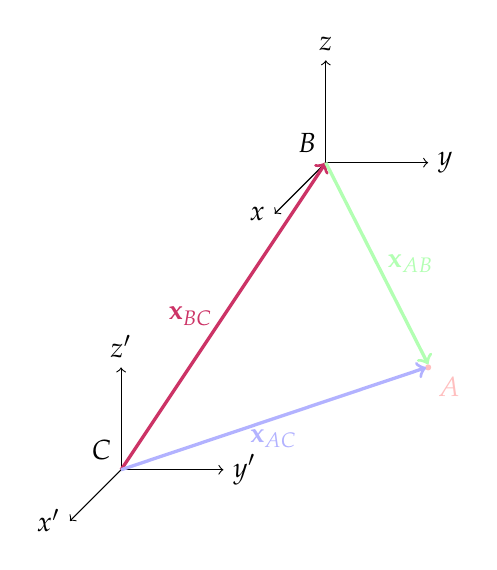
\begin{tikzpicture}[scale=1.3]
      \draw[->](0,0)--(-.5,-.5) node[pos=1,left]{$x'$}
      node[pos=0,above left]{$C$};
      \draw[->](0,0)--(1,0)     node[pos=1,right]{$y'$};
      \draw[->](0,0)--(0,1)     node[pos=1,above]{$z'$};

      \draw[->](2,3)--(1.5,2.5) node[pos=1,left]{$x$}
      node[pos=0,above left]{$B$};
      \draw[->](2,3)--(3,3)     node[pos=1,right]{$y$};
      \draw[->](2,3)--(2,4)     node[pos=1,above]{$z$};
      
      \draw[very thick,->,purple!80](0,0)--(2,3)
      node[midway,left]{$\mb{x}_{BC}$};
      \fill[pink] (3,1) circle(.03) node[below right]{$A$};
      \draw[very thick,->,blue!30](0,0)--(2.98,.998)
      node[midway,below]{$\mb{x}_{AC}$};
      \draw[very thick,->,green!30](2,3)--(3,1.03)
      node[midway,right]{$\mb{x}_{AB}$};
    \end{tikzpicture}

    \column{.6\textwidth}
    The position vector of the origins of the two reference frames is given by
    $\textcolor{purple!80}{\mb{x}_{BC}}$
    \begin{itemize}
    \item The vector pointing from the origin of frame $C$ to the origin of
      frame $B$
    \item If the two frames are moving relative to each other, then
    $\textcolor{purple!80}{\mb{x}_{BC}}$ is also a function of time
    \end{itemize}
    Without using vector notations, the relationship between the
    vectors is obvious:

    \eq{-.3in}{
      \boxed{
        \textcolor{blue!70!black}{\mb{x}_{AC}}=
        \textcolor{green!80!black}{\mb{x}_{AB}}+
        \textcolor{purple!80}{\mb{x}_{BC}}
      }
    }
  \end{columns}
\end{frame}



\begin{frame}{Relative Motion}
  \begin{columns}
    \column{.4\textwidth}
    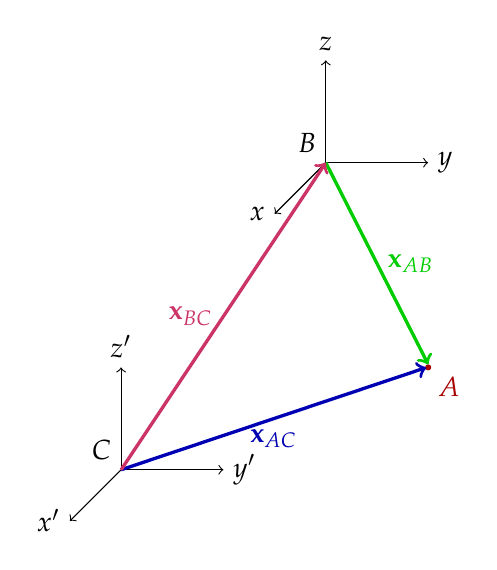
\begin{tikzpicture}[scale=1.3]
      \draw[->](0,0)--(-.5,-.5)  node[pos=1,left]{$x'$}
      node[pos=0,above left]{$C$};
      \draw[->](0,0)--(1,0) node[pos=1,right]{$y'$};
      \draw[->](0,0)--(0,1) node[pos=1,above]{$z'$};

      \draw[->](2,3)--(1.5,2.5)
      node[pos=1,left]{$x$}
      node[pos=0,above left]{$B$};
      \draw[->](2,3)--(3,3) node[pos=1,right]{$y$};
      \draw[->](2,3)--(2,4) node[pos=1,above]{$z$};

      \fill[red!65!black] (3,1) circle(.03) node[below right]{$A$};
      \draw[very thick,->,blue!70!black](0,0)--(2.98,.998)
      node[midway,below]{$\mb{x}_{AC}$};
      \draw[very thick,->,green!80!black](2,3)--(3,1.03)
      node[midway,right]{$\mb{x}_{AB}$};
      \draw[very thick,->,purple!80](0,0)--(2,3)
      node[midway,left]{$\mb{x}_{BC}$};
    \end{tikzpicture}

    \column{.6\textwidth}
    Starting from the definition of \textbf{relative position}:

    \eq{-.33in}{
      \boxed{
        \textcolor{blue!70!black}{\mb{x}_{AC}}=
        \textcolor{green!80!black}{\mb{x}_{AB}}+
        \textcolor{purple!80}{\mb{x}_{BC}}
      }
    }
    
    \vspace{-.1in}Using the definitions for velocity to get a similar
    equation for \textbf{relative velocity}:

    \eq{-.25in}{
      \boxed{
        \textcolor{blue!70!black}{\mb{v}_{AC}} =
        \textcolor{green!80!black}{\mb{v}_{AB}}+
        \textcolor{purple!80}{\mb{v}_{BC}}
      }
    }

    \vspace{-.1in}and \textbf{relative acceleration}:

    \eq{-.25in}{
      \boxed{
        \textcolor{blue!70!black}{\mb{a}_{AC}}=
        \textcolor{green!80!black}{\mb{a}_{AB}}+
        \textcolor{purple!80}{\mb{a}_{BC}}
      }
    }
  \end{columns}
\end{frame}



%\begin{frame}{Relative Velocity Example}
%  If an airplane ($P$) flies in windy air ($A$) we must consider the velocity
%  of the airplane relative to air, i.e.\ $\mb{v}_{PA}$ and the velocity of the
%  air relative to Earth $E$, i.e.\ $\mb{v}_{AE}$. The velocity of the airplane
%  relative to Earth is therefore
%
%  \eq{-.2in}{
%    \mb{v}_{PE}=\mb{v}_{PA}+\mb{v}_{AE}
%  }
%
%  \textbf{Simple example:} If an airplane is flying at a constant velocity of
%  \SI{253}{km/h} south relative to the air and the air velocity is
%  \SI{24}{km/h} east, what is the velocity of the airplane relative to Earth?
%\end{frame}



\begin{frame}{Relative Velocity}
  In classical mechanics, the equation for relative velocities follows the
  \textbf{Galilean velocity addition rule}, which applies to speeds much less
  than the speed of light:

  \eq{-.25in}{
    \mb{v}_{AC}=\mb{v}_{AB}+\mb{v}_{BC}
  }

  The velocity of $A$ relative to reference frame $C$ is the velocity of $A$
  relative to reference frame $B$, plus the velocity of $B$ relative to $C$. If
  we add another reference frame $D$, the equation becomes:

  \eq{-.25in}{
    \mb{v}_{AD}=\mb{v}_{AB}+\mb{v}_{BC}+\mb{v}_{CD}
  }
\end{frame}


\begin{frame}{Typical Problems}
  In the AP Physics 1 exam, kinematics questions appear in
  both multiple-choice and free-response sections. The problems themselves
  are not necessarily very different from Grade 11/12 Physics problems, but:
  \begin{itemize}
  \item You have to solve problems faster because of time constraint
  \item You can use $g=\SI{10}{\metre/\second\squared}$ in your calculations to
    make your lives simpler
  \item Many problems are \emph{symbolic}, which means that they deal with
    the algebraic expressions, not actual numbers
  \item Often coupled with other types (e.g.\ dynamics and rotational) in
    the free-response section
  \item You \emph{will} be given an equation sheet
  \end{itemize}
\end{frame}
\end{document}
